\documentclass[12pt,a4]{article}

\usepackage{graphicx,subfigure,a4wide,noparindent}

\title{Complex Gabor filters}
\author{Bill Christmas}

\begin{document}

\maketitle

In order to detect texture in scenes, the human visual system uses a set of bandpass filters that vary in orientation and centre frequency.  A Gabor filter bank is a set of regularly spaced filters that attempt to mimic this behaviour.  Typical filters might have point spread functions such as:

\begin{center}
  
\includegraphics{psf}  \hspace{2cm} 
\includegraphics{psf45}
\end{center}

Taking the first example as our prototype, such a filter has a point spread function of the form:

\[ g(x,y) = {1 \over 2 \pi  \sigma_r\sigma_\theta}\;
\exp \left\{ -{1\over2} \left[{\left(x\over\sigma_r\right)^2+\left(y \over \sigma_\theta\right)^2}\right]\right\} \;
\cos\left(2\pi U x\right) \]

The exponential term defines a Gaussian-shaped envelope of elliptical shape, and the cosine term defines the centre frequency.  The Gaussian envelope shape is used to get the best compromise of minimising the filter width in both spatial and frequency domains.  The problem with such a p.s.f.\ is that the response ripples in a similar manner to the cosine term in the p.s.f.  A convenient way to deal with this is instead to use a complex p.s.f.:

\[ g(x,y) = {1 \over 2 \pi  \sigma_r\sigma_\theta}\;
\exp \left\{ -{1\over2} \left[{\left(x\over\sigma_r\right)^2+\left(y \over \sigma_\theta\right)^2}\right]\right\} \;
\exp\left(i2\pi U x\right) \]
and to deal with the resulting complex filtered image by taking its modulus.  This gives a final response whose shape is influence by the Gaussian envelope of the p.s.f.\ instead of the p.s.f.\ itself.

The Fourier transform of the p.s.f.\ is given by:
\begin{equation}
  G(u,v) = \exp \left\{ -2\pi\left[ \sigma_r^2 (u-U)^2 +\sigma_\theta^2 v^2 \right] \right\}\label{eq:G}
\end{equation}
--- i.e.\ an elliptical shape whose centre is offset on the $u$ axis by the centre frequency $U$.

The frequency coordinate system can then be rotated and scaled to create an array of filters of $N$ different orientations and $M$ different scales, using the substitution:

\[ {u \choose v} = s^m \left( \begin{array}{rr}\cos \pi{n\over N} & \sin \pi{n\over N} \\ -\sin \pi{n\over N} & \cos \pi{n\over N} \end{array}\right) {u' \choose v'} ,\; m = 0, 1, \ldots, M-1,\; n = 0, 1, \ldots N-1,\; s > 1 \]
The scale ratio parameter $s$ thus defines the ratio of the centre frequencies of filters of adjacent scales, and also of their widths. 

The result is a set of filters that covers one half of the complex frequency plane, shown in Fig.~\ref{fig:spectrum}.  (We do not populate the lower half of the plane because the extra filters would have the same response as the existing ones.)  The set of filters can be made a little more compact by offsetting every other scale by $1\over 2$ of the angular separation (here the middle of the 3 scales), shown in Fig.~\ref{fig:shifted}.  Note however that this will reduce the number of filters that explicitly detect perceptually important vertical lines.
\begin{figure}[t]\centering
  \subfigure[no offset]{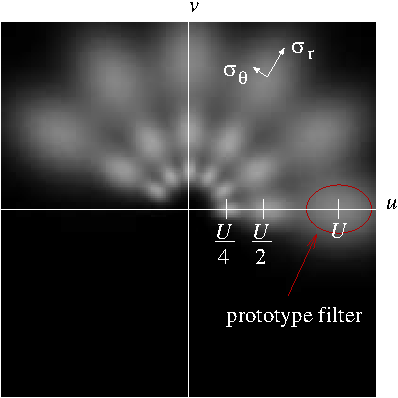
\includegraphics{maskfig}\label{fig:spectrum}}
  \hspace{2em}
  \subfigure[with alternate scales offset]{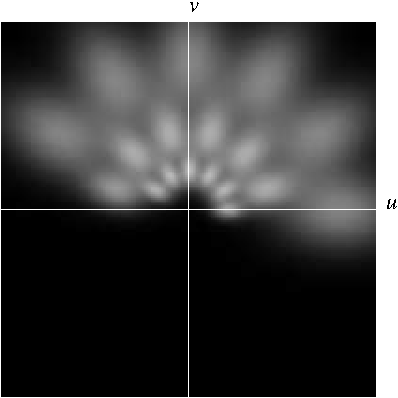
\includegraphics{offsetfig}\label{fig:shifted}}
  \caption{Spectral representation of filters: $M=3$, $N=6$, $s=2$\label{fig:spectra}}
\end{figure}

The filter scale parameters are set as follows.  Note that $\sigma_\theta$, $\sigma_r$ are the filter scales in the {\em spatial} domain.  

\paragraph{$\mathbf{\sigma_\theta}$:} 
This represents the filter scale in pixels in the tangential direction of the highest frequency filters.  It is more or less inversely proportional to the tangential filter separation.  Half-way between the centres of two filters adjacent in the tangential direction, the filter responses are equal ($=\delta$, say where $\delta < 1$). The distance between the two filters is given by (Fig.~\ref{fig:circles})
\def\Sinpbnn{\sin{\left(\pi\over2N\right)}}
\[ 2r = 2U \Sinpbnn \]
Since  $\delta$ is the response of a filter at a distance $U\sin(\pi/2N)$ from its centre in what is approximately the tangential direction, and $u$ is constant in the tangential direction ($u = U$ for the highest frequency filters), then from (\ref{eq:G}):

\[ \delta = \exp \left[ -2\pi \left(\sigma_\theta U \Sinpbnn\right)^2  \right] \]
\[ \rightarrow\quad \sigma_\theta =
  \sqrt{-\ln\delta \over 2\pi}\; {1 \over U\Sinpbnn} 
\]

Using $\delta = {1\over2}$ gives a reasonably uniform overall coverage of the spectrum in the tangential direction, in which case:
\[ \sigma_\theta \approx {1 \over 3 U\Sinpbnn} \]

\paragraph{$\mathbf{\sigma_r}$, no offsetting:}
$\sigma_r$ represents the filter scale in the radial direction of the highest frequency filters (the outer semi-ring in Fig.~\ref{fig:spectra}).  If we do not offset alternate scales (Fig.~\ref{fig:spectrum}), $\sigma_r$ and $\sigma_\theta$ are independent, so $\sigma_r$ depends only on the radial filter separation, which is a function of the scale ratio $s$.  The responses $\delta$ of the two outermost radially adjacent filters are equal when
\[ \exp\left[ -2\pi \sigma_r^2 (u-U)^2\right]
= \exp\left[ -2\pi \sigma_r^2 \left(su-U\right)^2\right] = \delta \]
%\[\rightarrow\quad (u-U)^2 = (su-U)^2 = {-\ln{\delta} \over 2\pi \sigma_r^2} \]

Selecting appropriate roots:
\begin{eqnarray}
   \sigma_r &=& \sqrt{-\ln{\delta}\over 2\pi} \;{s+1\over U(s-1)} \label{eq:sigma_r}\\
   &=& {s+1\over s-1}\; \Sinpbnn\; \sigma_\theta \nonumber
\end{eqnarray}
For $\delta={1\over2}$:
\[ \sigma_r \approx {s+1\over 3U(s-1)} \]
 
\paragraph{$\mathbf{\sigma_r}$, with offsetting:}
When alternate scales are offset by one half of the filter width (Fig.~\ref{fig:shifted}) the situation is more complicated.  Consider first the case when the filters are circular, i.e.\ 
\begin{equation}
  \label{eq:circ}
  \sigma_r = \sigma_\theta
\end{equation}

From basic geometrical properties (Fig.~\ref{fig:circles}), we can see that 
\[ \alpha + \beta = {N+1\over 2N}\pi, \quad \sin\alpha = {s_c\over 1+s_c}, \quad \cos\beta = {1\over 1+s_c} \]
where $N$ is the number of filters at the same scale, and $s=s_c$ is the scale ratio required to generate circular filters.
\begin{figure}
  \centering
  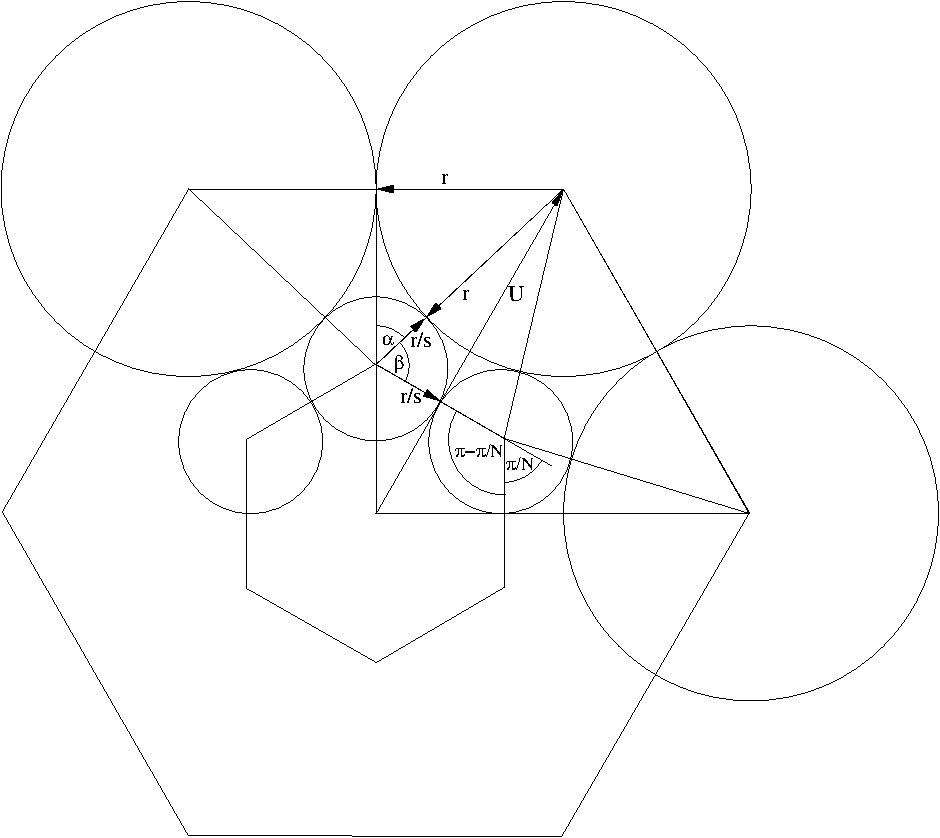
\includegraphics[width=0.6\textwidth]{circles}
  \caption{Geometry for circular Gabor filters; $N = 3$}
  \label{fig:circles}
\end{figure}

Defining $\tau = \sin\left({N+1\over 2N}\right)$, we can solve for $s_c$:
\[ s_c = {1+\tau-\tau^2 \pm \sqrt{(1+2\tau)(1-\tau^2)}\over \tau^2} \]
The positive root is the required one; the negative one corresponds to $1\over s$. For $N=4$, $s \approx 2$.

In the general case, for a desired value of $s$ we can use (\ref{eq:sigma_r}), (\ref{eq:circ}) to determine an appropriate value for $\sigma_r$:
\[ \sigma_r = {s+1 \over s-1}\: {s_c-1 \over s_c+1}\: \sigma_\theta \]



\end{document}


we put 
\[ \sigma_r = {N_c\over N}\, \sigma_\theta
\approx \sqrt{-\ln \delta \over 2\pi} \;{\sqrt{2s+1}\over (s-1) U} \]
which for $s=2$, $\delta={1\over2}$, gives:
\[ \sigma_r \approx {0.74\over U} \]

 
